\documentclass[11pt]{article}
\usepackage{amsmath, amssymb, amsfonts}
\usepackage{geometry}
\usepackage{setspace}
\usepackage{physics}
\usepackage{graphicx}
\usepackage{float}
\geometry{margin=1in}
\usepackage{hyperref}

\onehalfspacing

\title{Modeling California Energy
Prices Using Markov Chains}
\author{Andres Efren Rocha Jayasinha}
\date{}

\begin{document}
\maketitle

\section{Purpose of the Notebook}

This notebook constructs a \emph{discrete-time stochastic model} for electricity prices using observed market data for every single pricing node recorded in the California Independent System Operator's (CAISO) Open Access Same-Time Information System (OASIS) from January to March of 2025.


\noindent The main goal is to get deeper insight into how pricing behaves in California and how this behavior overall fits into California having some of the highest energy prices in the nation.

\noindent \textbf{\textit{The notebook can be found here: \href{https://github.com/arochaja/CAISO_MARKOV}{CAISO MARKOV}}}

\section{The Data Set}

\noindent The data set consists of ~35 millions rows of data containing hourly Locational Marginal Price data from January 1st all the way to March 31st, recording in \$/MW. A snapshot of the compiled data frame after merging all CSVs can be found in Table 1.

\begin{table}[h!]
\centering
\begin{tabular}{llrcr}
\hline
\textbf{INTERVALSTARTTIME\_GMT} & \textbf{NODE\_ID} & \textbf{MW} & \textbf{OPR\_HR} & \textbf{PriceType} \\
\hline
2025-01-01 05:00:00+00:00 & 0096WD\_7\_N001 & 50.91579 & 22 & MED \\
2025-01-01 03:00:00+00:00 & 0096WD\_7\_N001 & 51.23666 & 20 & MED \\
2025-01-01 07:00:00+00:00 & 0096WD\_7\_N001 & 50.40439 & 24 & MED \\
2025-01-01 06:00:00+00:00 & 0096WD\_7\_N001 & 50.57005 & 23 & MED \\
2025-01-01 02:00:00+00:00 & 0096WD\_7\_N001 & 51.19425 & 19 & MED \\
\hline
\end{tabular}
\caption{Sample MW data for node 0096WD\_7\_N001}
\label{tab:mw_data_sample}
\end{table}

\section{Creating Markov Chains}

Rather than modeling prices as continuous values, the notebook partitions the real line into a finite number of \emph{price regimes}.
I defined the four intervals as:
\[
\begin{aligned}
\text{NEG}  &:= [-20, 0), \\
\text{LOW}  &:= [0, 40), \\
\text{MED}  &:= [40, 60), \\
\text{HIGH} &:= [60, 80).
\end{aligned}
\]

\section{Expected State Duration}

After constructing transition matrices for each Price Node we can do the following. Suppose the process is currently in state $i$.
At each time step, it:
\begin{itemize}
    \item remains in $i$ with probability $P_{ii}$,
    \item exits $i$ with probability $1 - P_{ii}$.
\end{itemize}

\noindent Thus, the number of consecutive time steps spent in state $i$ follows a \textbf{geometric distribution} with success probability $1 - P_{ii}$.

\noindent The expected duration is therefore:
\[
\mathbb{E}[\text{duration in } i]
=
\frac{1}{1 - P_{ii}}.
\]

\noindent This quantity is computed for each price regime to quantify how long prices on average persist before changing regime.

\section{Figures}

\begin{figure}[H]
    \centering
    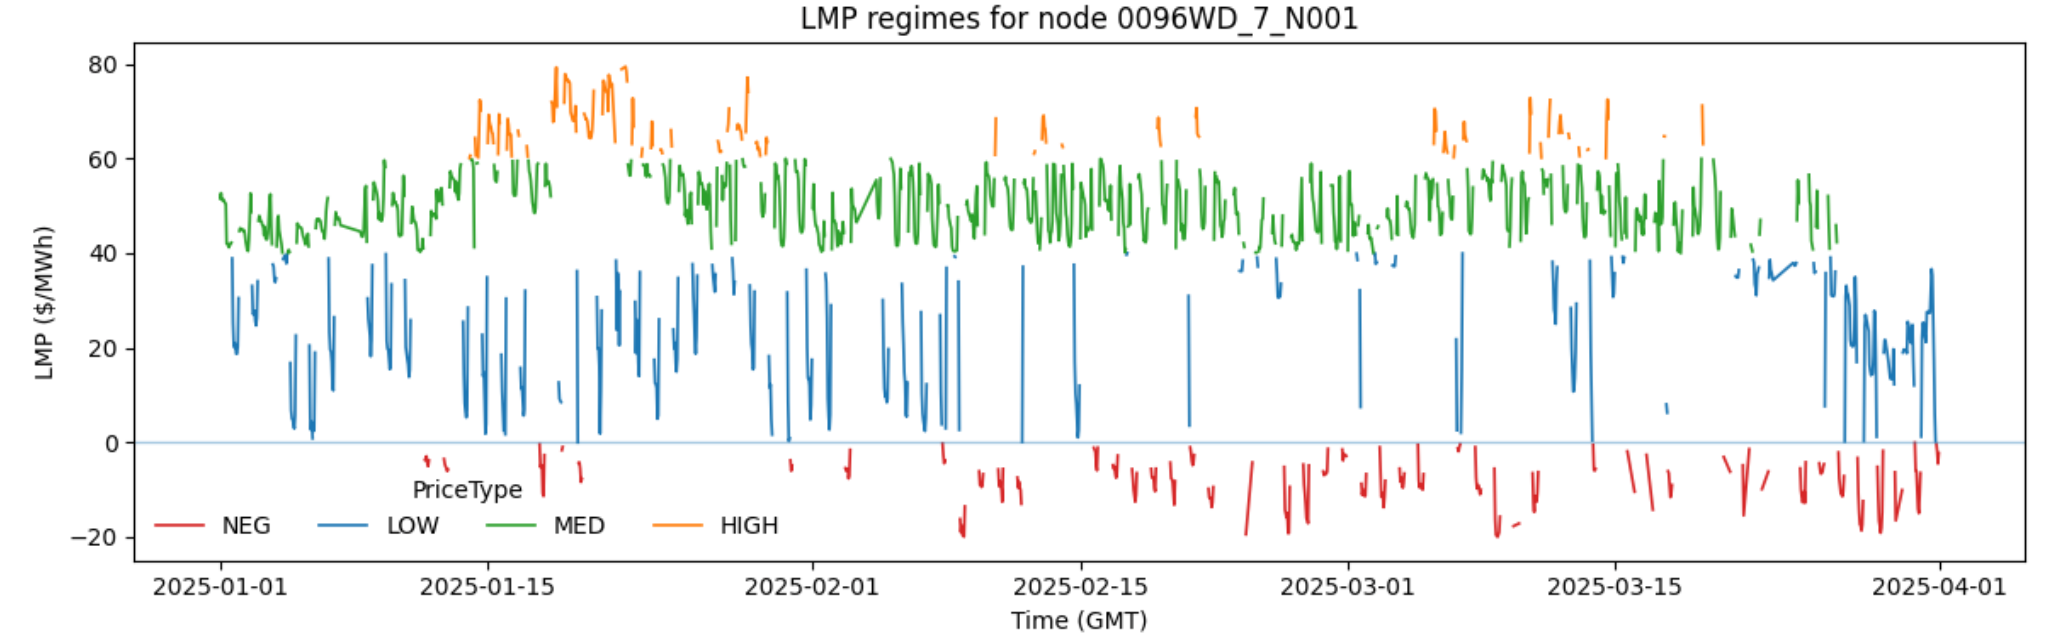
\includegraphics[width=1.0\linewidth]{figures/lmp-regimes-timeseries.png}
    \caption{This is a time series for a node with ID 009WD\_7\_N001 broken up by PriceType. The expected state durations computed were computed to be 5.22, 3.48, \textbf{6.42}, 3.24 hours for the Negative, Low, \textbf{Medium}, and High price regimes respectively. Notice how compared to the other price categories, the medium price threshold has the longest expected duration and also tends to be less interrupted in the time series.}
\end{figure}
    
\begin{figure}[H]
    \centering
    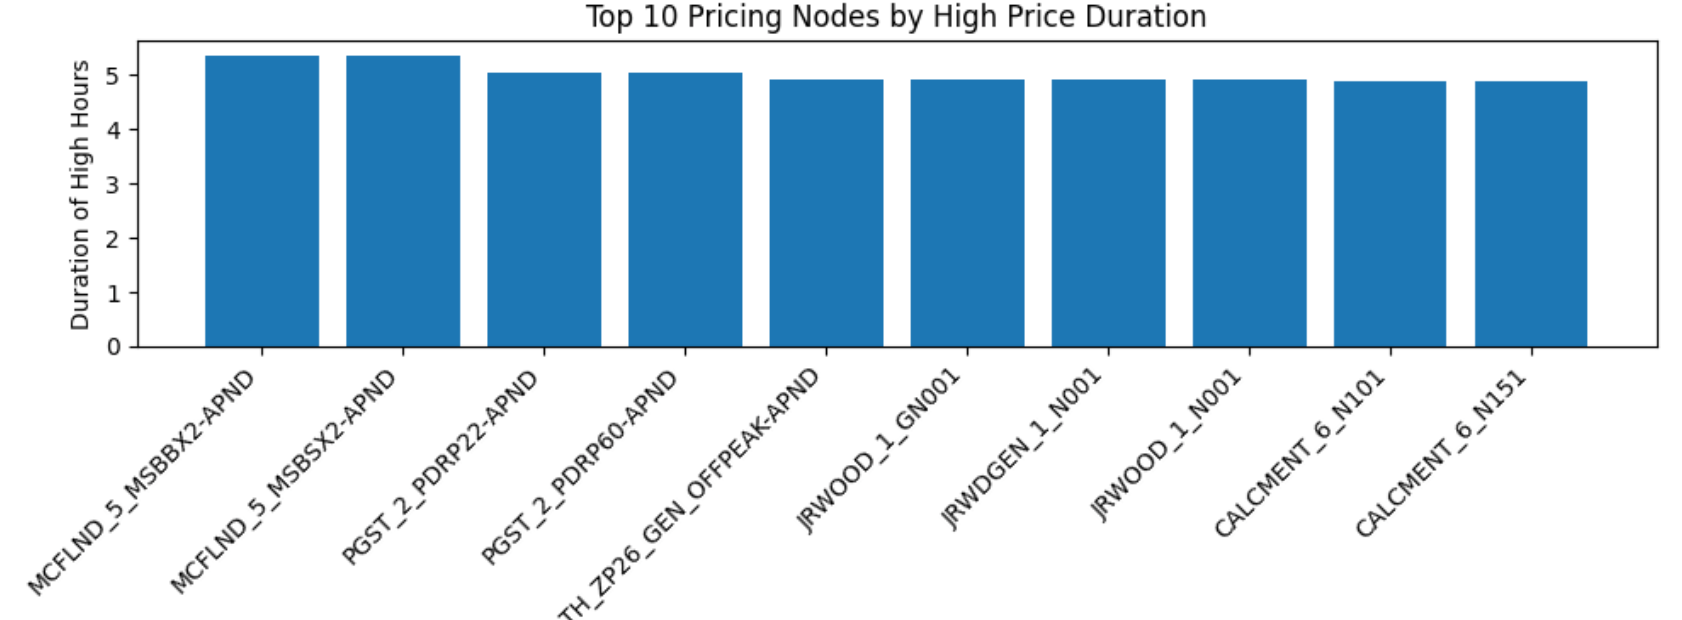
\includegraphics[width=1.0\linewidth]{figures/top10-nodes-high-price-duration.png}
    \caption{The expected state duration for high energy prices was computed. Pay special attention to the nodes with the tag ``MCFLND" denoting McFarland California.}
    \label{fig:high-price-duration}
\end{figure}

\begin{figure}[H]
    \centering
    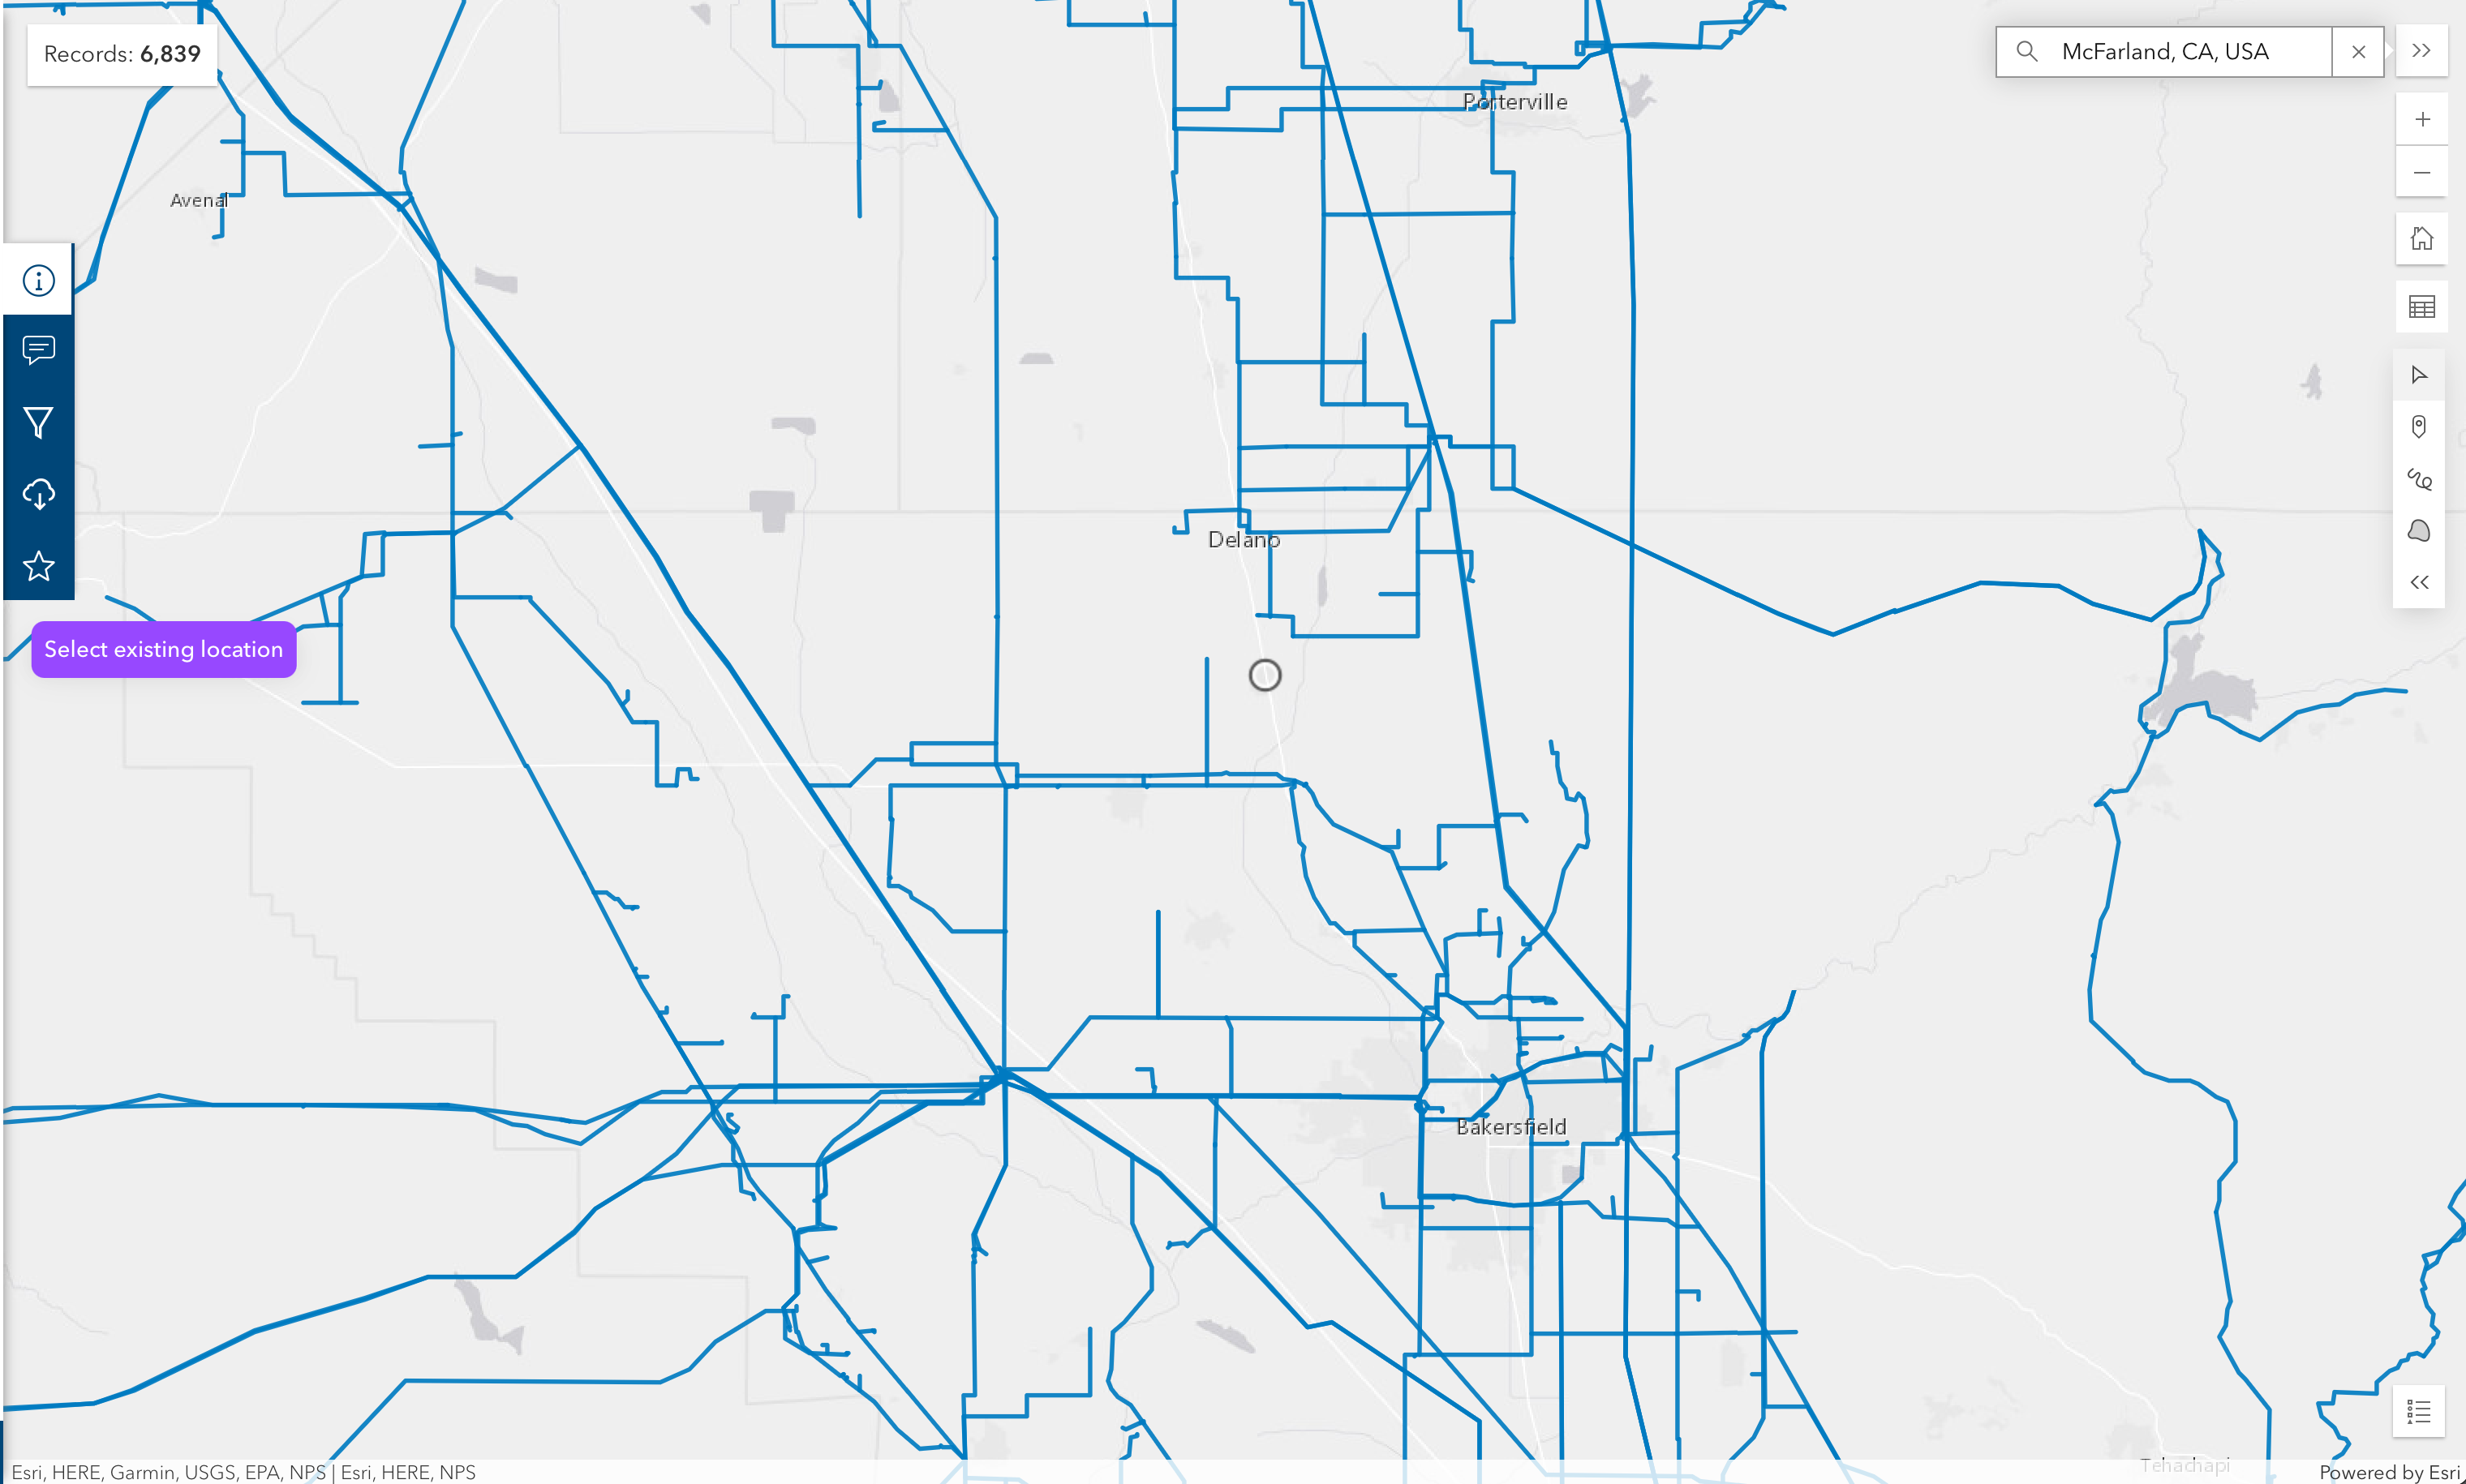
\includegraphics[width=0.8\linewidth]{figures/mcfarland-transmission-lines.png}
    \caption{The circle with gray outline is McFarland California and the blue lines represent transmission lines, notice the lack of transmission lines in its vicinity.}
    \label{fig:transmission-lines}
\end{figure}

\end{document}